        \section{Used scripts}

\subsection{Trees part}
To speed up trees coloring after calculating, I wrote a new script.
As input, it takes the best tree from MrBayes and adds a new tag (like probability, length, etc.) to leaves -- family.
Each family has its own identifier, so every representative sequence from it will have the same id.
This improved tree can be loaded in Figtree and using an internal tool, color by this tag.


To analyze the quality of the trees, I'm using another script that reads the standard deviation of split frequencies.
This data is presented on a plot (examples below).
Additionally, the plot can start from later generation (I'm using 1.000.000) to precisely show smaller values (Values before that point are unstable).

\subsection{Clustering}
To automate process of clustering low percentage Cd-Hit was used (psi-cd-hit).
Here two additional scripts were needed.
First is taking cd-hit .clstr file as input, and preparing files with groups.
User can also specify minimum of seequences in cluster to get qualified.
If this option is used, all small clusters are saved into one file.


Folder with group files and CLANS savefile are the input for the second script.
Script is reading inforamtions from CLANS savefile and writes a group section into it.
Sequences names need to exactly match those in savefile to be recognised.
As the point of the script is to use the same input file for CLANS clustering and those 2 scripts, there should be no issues.

\begin{figure}[H]
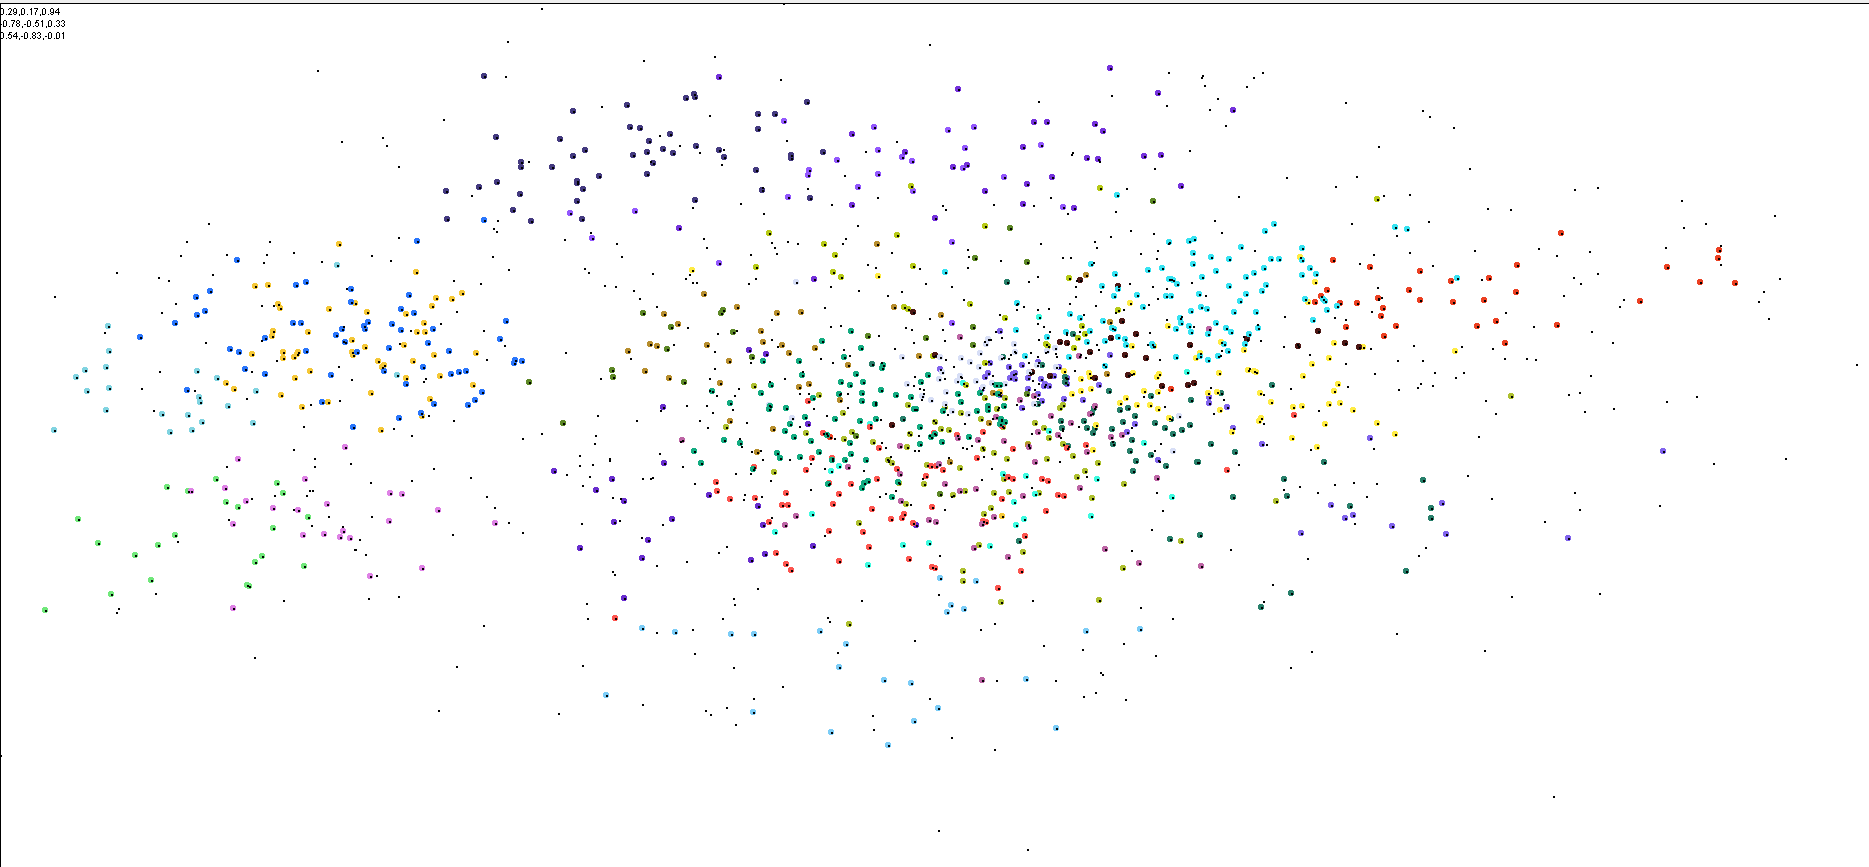
\includegraphics[width=\textwidth]{double-cd-hit-auto-cluster.png}
\caption{Example result of using those 2 scripts. Clustering of family PF01388.}
\end{figure}

